% IEEE-conference-template-062824 layout; original template remains unchanged.
% Manuscript maintained directly. Do not regenerate from the older Markdown outline.
\documentclass[conference]{IEEEtran}
\usepackage[T1]{fontenc}
\usepackage[utf8]{inputenc}
\usepackage{cite}
\usepackage{amsmath,amssymb,amsfonts}
\usepackage{graphicx}
\usepackage{booktabs}
\usepackage{balance}
\usepackage{textcomp}
\usepackage[hidelinks]{hyperref}
\begin{document}
\title{An Empirical Analysis of Categorical Search and Feature Selection in Recommender Fairness Testing}

\author{
\IEEEauthorblockN{Loo Pei Xin, Abdullateef Oluwagbemiga Balogun, Ahmad Sobri Hashim, Hussaini Mamman}
\IEEEauthorblockA{Department of Computing\\
Universiti Teknologi PETRONAS\\
Seri Iskandar, Malaysia\\
pei\_21000483@utp.edu.my, abdullateef.ob@utp.edu.my, sobri.hashim@utp.edu.my, hussaini@utp.edu.my}
}

\maketitle

\begin{abstract}
Feature selection changes which intersections a fairness audit can express, even when an optimizer successfully searches the remaining subgroups. We present a controlled empirical investigation of categorical subgroup search and feature-selection effects in recommender-system fairness testing. Established genetic algorithm (GA), ant colony optimization (ACO), differential evolution, artificial bee colony, and simulated annealing operators are compared with native double-ended discrete particle swarm optimization (DPSO), uniform random sampling, and exact enumeration where tractable. Synthetic experiments separate search behavior from recommendation utility; frozen-model audits cover MovieLens-1M, LFM360K, and a processed Amazon extract. On the evaluated synthetic landscapes, GA and ACO exceed native DPSO in mean maximum score. In MovieLens, random sampling already attains every exact full-grammar optimum, and enumeration needs only 294 evaluations, providing no evidence that adaptive optimization is necessary. The principal MovieLens finding concerns feature projection: 14, 18, and 15 observed above-threshold intersections reduce to 0, 0, and 1 with above-threshold projected parents across three checkpoints. This attenuation arises from backward elimination of audit attributes using activity-proxy labels and concerns that evaluated wrapper. Additional selection-target, subset-size, support, and dataset controls examine the scope of this effect. The contribution is empirical evidence about search and audit representation, with conclusions conditional on the evaluated models, metadata, and ranking protocols.
\end{abstract}

\begin{IEEEkeywords}
fairness testing, recommender systems, subgroup discovery, evolutionary computation, feature selection
\end{IEEEkeywords}

\section{Introduction}
\label{sec:introduction}

Recommender systems shape who receives useful recommendations, which items attract attention, and how opportunities are distributed across a platform. Evaluating these systems therefore requires considering the allocation of benefits among users, item providers, and other affected parties alongside aggregate predictive accuracy~\cite{burke2017multisided,biega2018equity,singh2018fairness}. Strong average ranking quality can coexist with systematically poorer recommendations for particular demographic groups. Prior work accordingly motivates explicit assessment of distributional differences as a distinct dimension of recommendation quality~\cite{yao2017beyond,beutel2019fairness}.

This assessment becomes more demanding when disadvantage occurs at demographic intersections. Users sharing several categorical attributes may experience disparities that are less apparent within broader groups. The resulting candidate space grows combinatorially, while sparse observations leave many combinations unsupported. Effective testing must therefore identify severe disadvantage and characterize how broadly it is distributed within the supported subgroup space.

FairRec searches for advantaged and disadvantaged groups using double-ended discrete particle swarm optimization~\cite{guo2023fairrec}. Its numerical movement rules use differences between nominal category codes, although those codes have no intrinsic distance. Incumbent-directed movement may also concentrate evaluations. We examine discovery breadth under these choices while retaining FairRec's thermal and double-ended exploration mechanisms.

FairAS targets general disadvantaged groups through adaptive sampling and local search~\cite{wu2025nobias}, motivating a persistent discovery archive alongside extreme-score reporting. A complementary challenge is reducing subgroup dimensionality without removing predicates needed to express disadvantage. Search policy and feature selection therefore require distinct evaluation.

Our central question is how feature selection affects fairness testing: can reducing the audit grammar obscure observed intersectional utility disparities even when search succeeds? We investigate this question through controlled subgroup comparisons, using established search algorithms as experimental instruments. The evaluated selection method applies Greedy Backward Elimination to the complete audit schema using development-user labels. In the original MovieLens experiment, these labels describe training activity rather than fairness outcomes. The analysis therefore concerns the projection induced by this predictive wrapper and whether observed intersectional signals survive it.

Calibration and exposure-opportunity measurements contextualize recommendation content. Causal and counterfactual discrimination require additional assumptions and intervention-based analysis~\cite{li2021towards,medda2024gnnuers}; longitudinal feedback also lies outside this static audit~\cite{mansoury2020feedback,zoralioglu2024dynamic}.

We ask: (RQ1) how do established search methods differ in attained severity and discovery breadth under matched request budgets; (RQ2) how much observed disparity survives feature projection, and how does this depend on selection target, subset cap, and support; and (RQ3) which observations extend to additional frozen-model datasets? The study separates synthetic search landscapes from real recommendation outcomes. MovieLens provides an exhaustively tractable demographic audit; supplementary LFM360K and Amazon audits examine additional metadata under a sampled-candidate protocol. Amazon's behavioral profiles are not protected demographic attributes. The paper makes three empirical contributions:
\begin{enumerate}
    \item A controlled comparison of five established heuristic challengers---GA, ACO, DE, ABC, and SA---against native DPSO and random sampling, with shared scoring, request accounting, and discovery measurements.
    \item A feature-projection analysis showing how the evaluated activity-proxy/backward-elimination pipeline can obscure observed MovieLens intersections, with selection-target, subset-size, and support ablations that bound the interpretation.
    \item Frozen-model audits across three datasets, using exact references and fixed-rule confirmation to distinguish optimizer attainment, expressible disparity, and outcome persistence. Negative optimizer findings are reported as empirical results.
\end{enumerate}

\section{Related Work}
\label{sec:related}

\subsection{Fairness Testing and Subgroup Discovery}
FairRec formulates fairness testing for deep recommenders across utility, item diversity, and item popularity, and introduces double-ended discrete particle swarm optimization to search for disadvantaged groups~\cite{guo2023fairrec}. Our study builds on this multi-perspective testing formulation and examines its search component using the native optimizer definitions with a controlled synthetic scoring oracle. This design isolates behavior on a specified landscape while keeping the scope distinct from replication of the original recommendation experiments.

FairAS targets general disadvantaged groups, motivating evaluation of discovery breadth in addition to an extreme score~\cite{wu2025nobias}. Our optional native adapter substitutes a categorical local-search hook within its adaptive driver; the portable mode implements a FairAS-inspired driver. Reporting these modes separately preserves the distinction between local-operator changes and changes to sampling, duplicate handling, or neighborhood construction.

\subsection{Categorical Search and Feature Selection}
Construction-based ACO represents a candidate as a sequence of discrete choices~\cite{dorigo1996ants}; GA recombines assignments across candidates. DE was developed for continuous optimization~\cite{storn1997de}; its use here requires an explicit random-key decoder. ABC~\cite{karaboga2007abc} and SA~\cite{kirkpatrick1983sa} add population-based categorical neighborhood search and a single-trajectory acceptance policy. These are established algorithm families. Our contribution is an empirical analysis of their search outcomes and of the subgroup signals retained after feature projection under explicit scoring and request policies.

Filter criteria such as mRMR balance feature relevance against redundancy~\cite{peng2005mrmr}, whereas wrappers evaluate candidate subsets through a predictive estimator. Our real-data study evaluates backward elimination from the complete audit schema. It asks whether the resulting projection preserves observed intersectional utility gaps; predictive feature relevance alone does not establish that preservation.

\subsection{Recommendation Calibration and Exposure}
NeuMF combines generalized matrix factorization and neural interaction modeling~\cite{he2017ncf}. Its predictions provide the recommendation slates audited here. Preference calibration has previously been studied as a recommendation objective~\cite{steck2018calibration}. Building on this motivation, our subgroup audit measures historical versus recommended genre distributions using Jensen--Shannon divergence. This defines the diagnostic used in our framework independently of the optimization formulation in the original calibration study.

Exposure fairness in rankings depends on an explicitly justified comparison target~\cite{singh2018fairness}. Our exposure-opportunity metric compares genre exposure with each user's eligible-catalog genre distribution. This user-level category-distribution diagnostic complements provider-oriented exposure formulations by making its eligible-catalog reference explicit. Calibration and exposure-opportunity measurements extend the framework's behavioral reporting through established auditing concepts.

\section{Methodology}
\label{sec:methodology}

\subsection{Recommender System and Objective Formulation}
We audit a frozen PyTorch Neural Matrix Factorization (NeuMF) recommender~\cite{he2017ncf}. Per-user NDCG@$K$ or Recall@$K$ supplies utility; the model, ranking protocol, and eligible items are fixed across search methods.

MovieLens supplies a diagnostic case study: its three-attribute full grammar has 294 cells and is exhaustively tractable. The 24-attribute synthetic experiments supply controlled high-dimensional search evidence, while two additional frozen-model datasets examine other metadata and supported densities. The study does not establish general real-model scalability or a universal heuristic advantage.

Let $\mathcal{U}$ be the audit population and $q_m(u)$ user $u$'s utility under metric $m$. A subgroup conjoins one category per retained attribute, stored as category indices or equivalent concatenated one-hot blocks. Category codes imply no demographic distance.

For a subgroup $g$ with membership set $\mathcal{U}_g$, we define its signed utility disparity as
\begin{equation}
\label{eq:utility-gap}
\Delta_m(g)=\overline{q}_m(\mathcal{U})-\overline{q}_m(\mathcal{U}_g),
\end{equation}
where, for any nonempty user set $A$,
\begin{equation}
\overline{q}_m(A)=\frac{1}{|A|}\sum_{u\in A}q_m(u).
\end{equation}
Positive values indicate that the subgroup receives lower recommendation utility than the global average. The primary search objective is
\begin{equation}
\label{eq:search-objective}
g^{*}=\underset{g:\,|\mathcal{U}_g|\geq n_{\min}}{\operatorname{arg\,max}}\;\Delta_m(g),
\end{equation}
where $n_{\min}$ excludes empty and insufficiently supported groups. This global-reference objective is an adaptation of the testing formulation and is distinguished from FairRec's range between extreme subgroup scores. Discovery uses validation interactions; selected subgroup rules are subsequently evaluated using held-out test interactions.

\subsection{Feature Selection and Audit Projection}
\label{sec:feature-selection}
The evaluated real-data selection method is Greedy Backward Elimination starting from the complete audit schema. We compare its selected grammar with the grammar containing all available audit attributes. This comparison measures the effect of removing predicates on expressible utility disparities; it does not evaluate a filter-fusion method.

The wrapper predicts development-user labels from categorical audit attributes using a one-hot encoded decision tree and cross-validated balanced accuracy. The original MovieLens labels indicate training activity below the development median, a proxy rather than a fairness outcome. Alternative MovieLens ablation arms and the additional-dataset audits use development-only labels indicating a utility deficit of at least 0.02 relative to the development mean. These dichotomized per-user labels are not continuous subgroup-disparity or causal-discrimination labels.

At each step, the wrapper evaluates all single-attribute deletions and chooses the deletion with the highest cross-validated predictive score, breaking ties by attribute order. Deletions are required until the maximum subset size is met. Thereafter, elimination stops if the best deletion would reduce the current score by more than the specified tolerance, or when the minimum subset size is reached. The cap is therefore an upper bound rather than a prescribed final size. Section~\ref{sec:experimental-setup} reports the estimator, folds, tolerance, and size constraints. Final confirmation outcomes do not determine selection settings.

The ablations compare no selection, alternative development targets, and subset-size caps. They assess this wrapper and the resulting projection, without attributing an effect to an unevaluated selection component. Predictive performance on development labels does not guarantee retention of intersectional fairness signals.

Feature removal changes the subgroup predicates available to the search, while eliminated attributes remain unconstrained. The audit population, recommender, utility metric, and global utility reference remain fixed. Consequently, feature selection reduces the dimensionality of subgroup discovery without redefining the comparison population.

\subsection{Categorical Search Adapters}
FairRec employs double-ended discrete particle swarm optimization (DPSO)~\cite{guo2023fairrec} to explore advantaged and disadvantaged subgroups. We investigate alternative operators because the inspected implementation constructs transitions using numerical differences between category codes, integer conversion, and boundary clipping. Nominal codes have no intrinsic distance, so equivalent category encodings can induce different numerical movements. Attraction toward incumbent solutions provides a second potential source of concentration, directing evaluations toward previously promising regions.

The evaluation examines representation sensitivity and discovery concentration while retaining FairRec's thermal and double-ended exploration.

The interchangeable GA adapter recombines attribute assignments through categorical crossover and introduces alternative values through mutation. These operators manipulate admissible categories without numerical distances between their codes.

ACO constructs assignments probabilistically, with one decision layer per attribute. Pheromone reinforcement favors promising choices; evaporation, bounded trails, and explicit exploration limit concentration. Neither adapter constitutes a new optimization algorithm; the contribution is their controlled integration and evaluation.

Three further established challengers broaden the empirical comparison. DE uses bounded random keys with per-attribute argmax decoding. ABC uses categorical donor moves, employed/onlooker phases, and charged scout restarts. SA uses one-coordinate category changes with geometric cooling. These are alternative search configurations, not additional algorithmic novelty. Random sampling and exhaustive enumeration establish whether adaptation yields a measurable advantage in a given grammar.

Comparisons fix subgroup semantics, support, and request budgets, while recording initialization differences. Repeats and invalid requests count. Outcomes include maximum disparity, distinct above-threshold groups, runtime, and observed stagnation.

An optional hybrid tester exposes the same operators through a FairAS local-search hook, with a shared request cap and persistent archive. Its mock integration checks are separate from the standalone comparisons reported here.

\subsection{Expanded Bias Auditing}
The framework supplements utility disparity with calibration and exposure-opportunity mismatch evaluators. These measurements characterize recommendation behaviors that aggregate NDCG or Recall gaps alone may not reveal.

For each user, calibration compares a category-preference distribution derived exclusively from training interactions with the rank-discounted category distribution of the recommendation slate. We quantify disagreement using base-2 Jensen--Shannon divergence:
\begin{equation}
\label{eq:calibration}
C(u)=\operatorname{JSD}_{2}\!\left(P_u^{\mathrm{history}},P_u^{\mathrm{slate}}\right).
\end{equation}
Exposure-opportunity mismatch compares the same slate distribution with a declared opportunity distribution, using total variation distance:
\begin{equation}
\label{eq:exposure}
E(u)=\frac{1}{2}\sum_c\left|P_u^{\mathrm{slate}}(c)-P_u^{\mathrm{opportunity}}(c)\right|.
\end{equation}
Opportunity uses the eligible-catalog category distribution. This is a descriptive reference; normative interpretations require a separately justified target.

The framework records subgroup/global means and signed/absolute gaps without changing utility fitness. Positive signed gaps indicate greater mismatch. Utility-selected groups need not reveal harms occurring only on another behavioral axis; those require a corresponding search objective.


Item mass is distributed across its genres; slate exposure uses normalized $w_r=1/\log_2(r+1)$. Opportunity averages genre mass over eligible items after ranking masks. Empty histories make calibration unavailable. Popularity and intra-list diversity are also logged, without novelty claims relative to FairRec. Audit rows follow utility-user order, with metric-specific valid counts.

\section{Experimental Setup}
\label{sec:experimental-setup}

\subsection{Evaluation Scope}
Synthetic scores assess categorical search; a separate real-model audit assesses recommendation utility and slates. Their score scales and evidence are kept distinct.

The initial synthetic comparison uses 24 attributes with cardinalities $(2,4,3)$ repeated eight times, landscape seed 2026, three searches per method, base search seed 42, population 20 per end, 4,000 requests, and threshold 0.65. All assignments are feasible.

Separately recorded post hoc controls add no model training or test-based tuning. They cross three score families, three seeded instances per family (2026--2028), three encodings (identity and two random relabelings), and five search seeds (1001--1005). The initial extension records five methods including uniform random (675 searches); a separately recorded revision adds ABC and SA under the same configuration (270 searches), totaling 945 searches at 4,000 requests each. Relabeling preserves semantic scores. Encodings and searches are not independent instances; threshold counts are interpreted within family.

Additive scores average independent seeded category weights in $[0,1]$. NK/trap scores combine mean three-attribute lookup values (weight 0.65) with planted triple rewards (weight 0.35): a full pattern match receives one, otherwise a triple with $h$ matches receives $(2-h)/3$. Modular scores count the fraction of eight disjoint triples whose semantic-category sum matches a seeded residue modulo three. Unequal category cardinalities can leave marginal associations, so this family is not claimed to contain only marginally invisible interactions.

\subsection{Dataset and Target Model}
The real-model experiment uses MovieLens-1M ratings, categorical user metadata, and movie genres. Ratings of at least four are treated as positive interactions, and users require at least three positives. The resulting checkpoint contains 6,035 users and 3,706 items.

For each user, the last two chronological positives form validation and test interactions; earlier positives form training data. NeuMF uses embedding dimension 16 and multilayer perceptron widths 64 and 32. Training uses Adam with learning rate $10^{-3}$, batch size 1,024, four sampled negatives per positive, and a 30-epoch cap. Development-user validation selects checkpoints with patience five and minimum improvement $10^{-4}$. For seeds 42, 100, and 2026, training stops after 25, 18, and 13 epochs, retaining checkpoints from epochs 20, 13, and 8, respectively. These are validation-selected checkpoints; the stopping rule does not establish mathematical convergence.

Users are partitioned once into 1,810 development users and 4,225 audit users using split seed 314159. Feature selection and checkpoint selection use development users; subgroup search uses validation interactions of audit users, followed by confirmation on their test interactions. The development/audit partition controls selection and evaluation; the recommender trains on earlier interactions from all eligible users.

Validation ranking excludes training positives; test ranking additionally excludes the validation positive. Evaluation uses full-catalog NDCG@10 with one held-out relevant item per user. Demographic attributes are used for auditing and do not enter the recommender.

\subsection{Baselines and Computational Controls}
The initial comparison evaluates native FairRec DPSO~\cite{guo2023fairrec}, categorical GA/ACO, and random-key DE. Every request counts, including repeats. Challengers share initial candidates and split budgets between maximizing and minimizing ends; native DPSO retains its initializer and coupled policy. Results therefore compare configurations, including initialization, under equal total requests.

The initial NeuMF comparison uses population 20, 4,000 requests per method/seed, support 20, and threshold 0.02. Three paired model/search seeds yield 12 successful runs. Cached search times exclude training and objective setup.

The initial demographic grammar contains gender, age, and occupation. Backward elimination starts from all three attributes and uses three-fold cross-validation and a depth-five decision tree, with at most two retained features. Labels indicate training activity below the development median (58 positives), a proxy rather than a measured fairness outcome. Eliminated attributes remain unconstrained.

For reproduction of the saved runs, the archived experimental code includes mRMR and Chi-square ranking hooks, each configured to retain the top ten attributes before taking their union. Each evaluated real-data schema has three attributes, so these hooks retain the entire schema and perform no reduction. They are disclosed solely as settings of our archived implementation and are omitted from the evaluated method in Section~\ref{sec:feature-selection}. The hooks belong to our experimental implementation; this study does not claim to reproduce a FairRec feature-selection pipeline. No mRMR, Chi-square, or fusion benefit is evaluated or claimed.

The checkpoint extension crosses ten independent search seeds (1001--1010) with each of the three frozen models. Native DPSO, GA, ACO, DE, and uniform random sampling are compared in both the original selected grammar and the unfiltered gender--age--occupation grammar, producing 300 searches. Each run retains the 4,000-request budget, population 20, support 20, and disparity threshold 0.02. Random sampling uses the challengers' initial candidates followed by independent uniform category assignments; repeats and invalid requests count. Exact enumeration separately scores every cell once, establishing within-grammar optima, regret, threshold recall, and optimum-attainment rates. It stops at space exhaustion rather than consuming an artificial 4,000 requests. The unfiltered space contains only 294 cells, so this is a correctness and selection audit rather than a scalability test.

The revision adds ABC and SA for all 60 model--grammar--search-seed combinations, bringing this comparison to 420 searches across seven methods. Earlier result folders are preserved; added indexed cell scores are checked against every original exact score before search. Cross-method runtimes from the two implementations are not pooled.

\subsection{Optimization Hyperparameters}
All heuristic challengers use 20 initial candidates per end and split 4,000 requests equally between maximizing and minimizing signed scores. Shared starts are sampled with NumPy SeedSequence $[s,0]$ and challenger search randomness with $[s,1]$. Cached duplicates, unsupported cells, and initialization consume requests; there is no early stopping or parameter tuning against test outcomes.

GA uses size-three tournaments, uniform crossover with probability 0.5 per coordinate, mutation probability $1/d$ per coordinate to a different category, and one cached elite. ACO starts trails at one, evaporates 20\% per batch, reinforces the best $\lfloor20/3\rfloor=6$ valid ants by $1/(r+1)$ for zero-based rank $r$, clips trails to $[0.05,20]$, and mixes trail sampling with 10\% uniform exploration; its heuristic is constant. DE uses DE/rand/1/bin random keys, differential weight 0.7, crossover 0.8 with one forced donor key, clipping to $[0,1]$, argmax decoding, and nonworsening replacement. ABC uses 20 employed and 20 rank-weighted onlooker attempts per complete cycle, one-coordinate donor moves, strict-improvement replacement, and abandonment after ten failed attempts. SA starts at the best initialized candidate per end, changes one coordinate, and cools geometrically from 0.15 to 0.001 over the remaining requests with Metropolis acceptance.

Native DPSO retains thermal coefficient 0.09, cognitive/social coefficients 2.0, velocities clipped to $[-2,2]$, integer position conversion, and category-bound clipping. Its uniform category initializer and coupled two-ended control flow remain native; equal budgets do not imply identical trajectories or starts. The generation cap is 4,000, with the request ledger enforcing the earlier total-request stop. Exhaustive evaluation ends at grammar exhaustion.

\subsection{Feature-Selection Ablation Design}
The MovieLens target-by-cap ablation crosses activity-proxy versus development-utility-deficit labels with maximum subset sizes two and three, retaining the unfiltered reference. At each checkpoint, exact scoring evaluates all five arms at supports 20, 50, 100, and 200 (60 cases). Backward elimination starts from the complete schema and uses three-fold stratified cross-validation, balanced accuracy, a one-hot encoded depth-five decision tree, minimum one feature, and tolerance 0.001. Caps are upper bounds, not required final sizes. This design examines target and wrapper-constraint effects jointly with support sensitivity.

\subsection{Additional Frozen-Model Datasets}
We audit the locally supplied FairRec-processed LFM360K and Amazon tables and frozen DeepFM checkpoints~\cite{guo2023fairrec,guo2017deepfm}. No additional model training is performed. All current model variables are verified as restored; unused optimizer slots are permitted. Embedding dimension is four; inference uses batches of 8,192 with four intra-operation threads and one inter-operation thread under Python 3.8.0, TensorFlow 2.3.0, and DeepCTR 0.9.3. Original checkpoint training seeds, stopping histories, and all preprocessing decisions cannot be reconstructed, so these are one-checkpoint supplementary audits per dataset.

Each supplied table contains one relevant item and 49 sampled negative rows per eligible user. We calculate per-user NDCG@10 on these 50 rows, ordering by descending predicted score and ascending item ID for ties; duplicate candidate rows are retained. These utilities are not comparable in level to MovieLens full-catalog NDCG. The eligible extracts contain 267,034 LFM360K and 175,878 Amazon users. LFM360K uses gender, age, and country. Amazon uses history level, mean-price level, and maximum-price level. These are behavioral profiles, not demographic protected groups; the supplied extract does not establish its original Amazon category/release or leakage-free history construction.

Using split seed 314159 separately within each table, 30\% of users form development, 35\% discovery, and the remainder confirmation, with integer counts rounded down for the first two partitions. The metadata vocabulary is declared from the supplied user table without using utility outcomes. Feature selection uses only development utility-deficit labels, with caps two and three. Discovery compares selected and unfiltered grammars at support 20 and threshold 0.02. Seven methods and ten search seeds give 140 searches per dataset (280 total), at 4,000 requests each. Both datasets have supported cells in both grammars, and exact enumeration supplies within-grammar references. Both caps and no selection are scored at supports 5, 20, 50, and 100 (24 ablation cases across the two datasets). One discovery-maximizing rule per grammar is fixed before confirmation on disjoint users; pointwise bounded-outcome intervals use the formula below. Disjoint confirmation users reduce outcome reuse but do not verify the supplied checkpoint's historical training separation or eliminate shared-model dependence.

\subsection{Projection and Fixed-Rule Confirmation}
To measure attenuation by feature removal, each supported above-threshold full cell is mapped to its selected-feature parent. We count how many full cells have parents that still exceed 0.02, keeping the audit users and global reference fixed; multiple cells may share one parent. This measures aggregation across eliminated attributes, not optimizer regret between equivalent grammars. In MovieLens, one exhaustive validation maximizer per model and grammar is fixed using enumeration order to break ties, then evaluated on test interactions. Exploratory pointwise intervals use 2,000 user-bootstrap resamples, preserving subgroup membership in the global reference. To guard against zero bootstrap variance in sparse zero-hit groups, we also report conservative bounded-outcome intervals. Writing $N$ for audit users, $n$ for subgroup support, and $p=n/N$, the gap is $(1-p)(\overline q_{\neg g}-\overline q_g)$. Two Hoeffding bounds and a union bound give a fixed-rule 95\% radius
\begin{equation}
(1-p)\left[\sqrt{\frac{\log 80}{2n}}+\sqrt{\frac{\log 80}{2(N-n)}}\right].
\end{equation}
This calculation assumes independent bounded user outcomes and fixes the observed group proportion. In MovieLens, neither interval adjusts for adaptive selection or multiplicity; shared audit users and post hoc design prevent interpreting them as independent population confirmation. Additional-dataset bounds use disjoint confirmation users but remain pointwise and conditional on the supplied checkpoint.

\subsection{Measurements}
We report attained maxima, first attainment, unique assignments, above-threshold breadth, invalid requests, and runtime. Progress uses objective requests rather than incompatible native generation counts.

Calibration and exposure-opportunity measurements accompany utility-selected groups without modifying fitness. These descriptive measurements complement the distinct explanatory and intervention-based questions addressed by counterfactual approaches~\cite{li2021towards,medda2024gnnuers}. The opportunity distribution is explicitly declared because exposure comparisons depend on the selected reference~\cite{singh2018fairness}.

Extension timings include cached objective scoring, optimization, and in-memory request recording; frozen-model inference and compressed trace output are excluded. They therefore differ from the original expanded-audit timings. Extension traces record every request, including duplicates and unsupported candidates. Category-permutation summaries report changes across recorded encodings; because encoded initial candidates are shared, rather than semantically coupled across encodings, these changes do not isolate numerical movement from initialization and finite-search randomness.

\section{Results and Discussion}
\label{sec:results}

\subsection{Initial Synthetic Comparison}
The initial three-run comparison on one NK/trap landscape yields mean maximum scores of 0.60838 for native DPSO, 0.71938 for GA, 0.72630 for ACO, and 0.73499 for DE. GA and ACO discover $405.0\pm83.4$ and $546.7\pm219.8$ distinct candidates above 0.65, compared with zero for DPSO. These are synthetic scores and category assignments, not measured population disparities. DPSO evaluates 381 distinct assignments on average, compared with 2,336.3 for GA and 3,570.3 for ACO. Its final best is first reached at requests 347, 3,035, and 2,303, which supports concentrated exploration but not a uniform early-collapse mechanism. These initial observations motivate the broader controls below.

\begin{table*}[t]
\centering
\caption{Synthetic comparison: 945 searches, with 45 per family/method. Each family lists mean maximum score, mean distinct candidates above 0.65 (breadth), and mean within-instance encoding spread. These are descriptive search outcomes on designed landscapes, not population utility disparities.}
\label{tab:synthetic-robustness}
\small
\begin{tabular}{lrrrrrrrrr}
\toprule
Method & Add. score & Breadth & Spread & NK score & Breadth & Spread & Mod. score & Breadth & Spread \\
\midrule
DPSO & 0.6278 & 0.8 & 0.0107 & 0.6090 & 0.3 & 0.0230 & 0.8861 & 16.4 & 0.0417 \\
GA & 0.7181 & 754.9 & 0.0000 & 0.7179 & 357.7 & 0.0124 & 1.0000 & 805.0 & 0.0000 \\
ACO & 0.7181 & 1023.1 & 0.0000 & 0.7187 & 409.9 & 0.0109 & 1.0000 & 546.8 & 0.0000 \\
DE & 0.7104 & 558.4 & 0.0031 & 0.7039 & 126.8 & 0.0160 & 1.0000 & 406.4 & 0.0000 \\
ABC & 0.7163 & 368.4 & 0.0025 & 0.6943 & 45.6 & 0.0107 & 1.0000 & 600.8 & 0.0000 \\
SA & 0.7180 & 538.9 & 0.0001 & 0.7228 & 251.6 & 0.0122 & 1.0000 & 801.4 & 0.0000 \\
Random & 0.6385 & 0.8 & 0.0074 & 0.6350 & 0.2 & 0.0144 & 0.9194 & 78.6 & 0.0500 \\
\bottomrule
\end{tabular}
\end{table*}

\subsection{Synthetic Robustness Across Families and Encodings}
The extension separates score-family effects from repetition on one landscape. Table~\ref{tab:synthetic-robustness} summarizes 945 searches across seven methods, with five search seeds crossed with three encodings of each of three instances per family. Breadth counts are compared within a family because the common threshold does not imply equivalent difficulty across score distributions. Encoding spread describes the range of encoding-specific mean maxima, averaged across instances; it does not estimate a causal effect of category arithmetic.

GA and ACO both attain mean maximum 0.71808 on additive instances, compared with 0.62778 for DPSO and 0.63854 for random sampling. On NK/trap instances, GA and ACO reach 0.71788 and 0.71868, versus 0.60898 for DPSO and 0.70386 for DE. Thus DE's highest mean in the initial three-run comparison does not persist in the expanded NK/trap design. On modular instances, GA, ACO, and DE all attain score one in every search, whereas DPSO and random sampling average 0.88611 and 0.91944.

Discovery breadth remains method- and family-dependent. ACO has the largest mean archive on additive and NK/trap instances (1,023.1 and 409.9 candidates), while GA leads on modular instances (805.0). These results support categorical adaptive search on the tested synthetic families, without identifying one universally best operator. On NK/trap instances, DPSO's mean encoding spread is 0.02297, compared with 0.01236 for GA, 0.01089 for ACO, and 0.01439 for random sampling. Variation even in random sampling emphasizes why a nonzero spread alone cannot establish a numerical-encoding mechanism.

The additional heuristics sharpen this qualification. SA reaches mean maximum 0.72280 on NK/trap instances, exceeding GA and ACO, whereas ABC reaches 0.69428. Both attain score one in every modular search; their modular breadths average 600.8 for ABC and 801.4 for SA. Thus GA/ACO performance relative to native DPSO does not justify claiming superiority over established heuristics generally. The contribution is a controlled characterization of these configurations and their tradeoffs between score and discovery breadth.

\subsection{Exact NeuMF References and Search Repeats}
\begin{table}[t]
\centering
\caption{MovieLens: 30 searches per method/grammar (ten seeds on three fixed models). Hit is exact-optimum attainment; recall is the fraction of supported above-threshold cells recovered, omitting cases with no such cells. Query is median first optimum request among successful searches. Timings from the earlier and indexed implementations are not pooled.}
\label{tab:extended-neumf}
\small
\begin{tabular}{llrrrr}
\toprule
Space & Method & Hit\% & Regret & Rec.\% & Query \\
\midrule
Sel. & DPSO & 100 & 0.00000 & 100.0 & 11.0 \\
Sel. & GA & 100 & 0.00000 & 100.0 & 4.0 \\
Sel. & ACO & 100 & 0.00000 & 100.0 & 4.0 \\
Sel. & DE & 100 & 0.00000 & 100.0 & 4.0 \\
Sel. & ABC & 100 & 0.00000 & 100.0 & 4.0 \\
Sel. & SA & 100 & 0.00000 & 100.0 & 4.0 \\
Sel. & Random & 100 & 0.00000 & 100.0 & 4.0 \\
Full & DPSO & 93 & 0.00077 & 64.6 & 32.0 \\
Full & GA & 100 & 0.00000 & 99.6 & 44.0 \\
Full & ACO & 100 & 0.00000 & 90.3 & 31.0 \\
Full & DE & 100 & 0.00000 & 89.0 & 51.5 \\
Full & ABC & 100 & 0.00000 & 99.8 & 37.0 \\
Full & SA & 100 & 0.00000 & 95.2 & 31.5 \\
Full & Random & 100 & 0.00000 & 100.0 & 36.0 \\
\bottomrule
\end{tabular}
\end{table}

All 210 selected-grammar searches attain an exact optimum. The selected spaces contain seven cells for model seeds 42 and 100 and fourteen for seed 2026. Their maximum gaps remain 0.01495, 0.01484, and 0.03669, respectively. Thus the original agreement across optimizers persists with independent search repeats and the added ABC/SA configurations.

The unfiltered gender--age--occupation grammar has 294 possible cells, of which 61 satisfy support 20. GA, ACO, DE, and random sampling attain exact optima in all 30 searches each. Native DPSO succeeds in 28 of 30, with mean regret 0.00077. Mean above-threshold recall is 64.6\% for DPSO, 99.6\% for GA, 90.3\% for ACO, 89.0\% for DE, and 100\% for random sampling. These are conditional search-repeat summaries on three fixed checkpoints, not independent dataset replications.

ABC and SA also reach all 30 full-grammar optima, with mean threshold recall 99.8\% and 95.2\%, respectively. Adding heuristics therefore broadens the comparison without changing the negative finding: none has an endpoint advantage over random sampling in this MovieLens setting.

The budget is over thirteen times the number of possible full cells, making random sampling a strong reference. Its median first optimum request is 36, compared with 32 for successful DPSO searches, 44 for GA, 31 for ACO, and 51.5 for DE. Figure~\ref{fig:attainment} shows the recorded attainment trajectories. First-hit summaries exclude failed searches and therefore must be read with attainment rates. Exact enumeration needs only 294 requests to establish every full-cell score, including invalid cells. Adaptive search has no demonstrated endpoint advantage over random or exhaustive evaluation in this small real-model domain.

The two references address different questions. Random sampling tests whether adaptive proposals improve discovery under the same charged budget; its complete threshold recall makes such a benefit unsupported here. Exhaustive enumeration certifies the attainable within-grammar gaps, rules out hidden search regret, and evaluates every cell in fewer requests than the heuristic budget. A uniform sampler's probability of visiting any particular full cell within $B$ independent requests is $1-(293/294)^B$, explaining why 4,000 requests make endpoint attainment a weak discriminator. Early-budget trajectories remain descriptive; a case for adaptive optimization would require a demonstrable advantage at smaller budgets or in substantially larger supported grammars.

\begin{figure}[t]
    \centering
    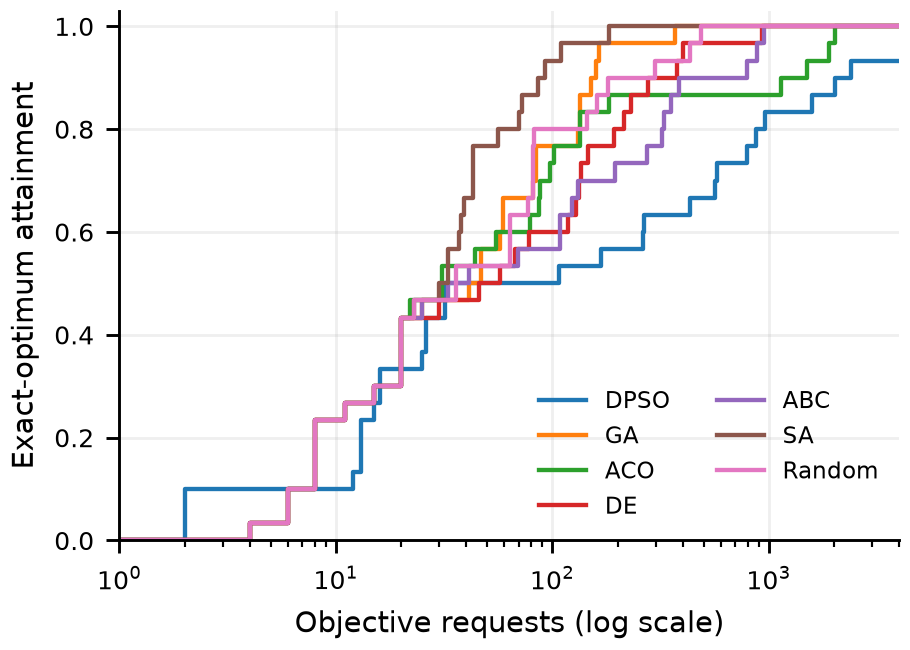
\includegraphics[width=\columnwidth]{assets/revision_attainment.png}
    \caption{Exact-optimum attainment in the unfiltered NeuMF grammar, using recorded first-hit requests. Each method has ten searches on each of three fixed checkpoints. Searches that fail to reach an optimum remain unattained at 4,000 requests.}
    \label{fig:attainment}
\end{figure}

\subsection{Feature Selection Attenuates Observed Gaps}
\begin{table}[t]
\centering
\caption{Selection audit against exhaustive full conjunctions (294 possible cells per model). Valid counts supported full cells; retained counts high-gap full cells whose selected-feature parent also exceeds 0.02. This is threshold attenuation under aggregation, not a same-grammar optimizer comparison.}
\label{tab:selection-ablation}
\small
\begin{tabular}{rrrrrr}
\toprule
Seed & Sel. & Valid & $\Delta_{sel}$ & $\Delta_{full}$ & Retained \\
\midrule
42 & 7 & 61 & 0.01495 & 0.04662 & 0/14 \\
100 & 7 & 61 & 0.01484 & 0.04378 & 0/18 \\
2026 & 14 & 61 & 0.03669 & 0.04497 & 1/15 \\
\bottomrule
\end{tabular}
\end{table}

Exact unfiltered maximum validation gaps are 0.04662, 0.04378, and 0.04497 for seeds 42, 100, and 2026. The selected maxima are smaller by 0.03166, 0.02894, and 0.00828, respectively. These differences reflect a change in expressible predicates, rather than search failure within an unchanged grammar.

More directly, the full audit finds 14, 18, and 15 supported intersections above 0.02. Mapping those cells to their selected-feature parents leaves 0, 0, and 1 parents above threshold. The corresponding high-gap full cells contain 652, 658, and 599 audit users; only 43 users in the third model belong to a high-gap full cell with an above-threshold parent. This comparison measures attenuation by aggregation, without treating threshold flags as confirmed population harms.

The ablation supplies evidence against assuming that activity-based predictive selection preserves utility-disadvantage signals. The observed reduction is determined by backward elimination from all three audit attributes. The appropriate conclusion is that the evaluated activity-proxy wrapper can conceal observed intersectional gaps, even while simplifying optimization. A practical audit should enumerate a tractable full grammar and evaluate gap retention before accepting a projected grammar; predictive activity accuracy alone is insufficient evidence of that retention.

\subsection{Selection-Target, Subset-Size, and Support Ablations}
\begin{table*}[t]
\centering
\caption{MovieLens target-by-cap ablation at support 20: exact maximum gap and, in parentheses, high full cells with an above-threshold parent divided by all high full cells. A/U denote activity/utility-deficit targets; 2/3 are maximum subset sizes. Each selection arm applies backward elimination from the complete audit schema.}
\label{tab:target-ablation}
\small
\begin{tabular}{rlllll}
\toprule
Seed & A2 & A3 & U2 & U3 & Full \\
\midrule
42 & 0.0150 (0/14) & 0.0466 (14/14) & 0.0150 (0/14) & 0.0150 (0/14) & 0.0466 (14/14) \\
100 & 0.0148 (0/18) & 0.0148 (0/18) & 0.0274 (3/18) & 0.0274 (3/18) & 0.0438 (18/18) \\
2026 & 0.0367 (1/15) & 0.0367 (1/15) & 0.0226 (1/15) & 0.0226 (1/15) & 0.0450 (15/15) \\
\bottomrule
\end{tabular}
\end{table*}

Table~\ref{tab:target-ablation} compares activity and utility-deficit targets under caps two and three. For seed 42, relaxing the activity cap retains all three attributes and all 14 above-threshold full cells, whereas utility-target selection retains age alone and none of those cells under either cap. For seed 100, utility-target selection retains occupation and preserves 3 of 18 full-cell flags, compared with none under activity selection. For seed 2026, both targets preserve only 1 of 15 flags, despite different selected grammars. A utility-related label therefore does not by itself guarantee retention of intersectional utility gaps, and a relaxed cap is not a requirement to retain every attribute.

Support sensitivity supplies a second boundary. Raising the full-grammar support threshold from 20 to 50, 100, and 200 leaves 61, 19, 8, and 1 supported cells, respectively, for each MovieLens checkpoint. The above-threshold counts change from 14/18/15 at support 20 to 6/4/4 at 50, 1/1/1 at 100, and 0/0/0 at 200. This is a change in the population intersections admitted to the audit, not evidence that higher support removes underlying harms. These controls remain post hoc and concern the specified wrapper and support policy.

\subsection{Additional Datasets: Projection and Search}
\begin{table*}[t]
\centering
\caption{Additional frozen DeepFM audits at support 20. Users are development/discovery/confirmation; cells are total/supported full conjunctions; retained counts full high-gap cells whose selected parent remains above 0.02. Selected features use development-utility labels and a two-feature cap.}
\label{tab:additional-datasets}
\small
\begin{tabular}{llrlrrr}
\toprule
Dataset & Users (D/A/C) & Full cells & Selected predicates & $\Delta_{full}$ & $\Delta_{sel}$ & Retained \\
\midrule
LFM360K & 80,110/93,461/93,463 & 53,058/894 & gender, country & 0.2511 & 0.1173 & 115/323 \\
Amazon & 52,763/61,557/61,558 & 1,000/325 & history, max price & 0.1699 & 0.0878 & 15/84 \\
\bottomrule
\end{tabular}
\end{table*}

\begin{table*}[t]
\centering
\caption{Additional datasets: exact-optimum hit rate / mean above-threshold recall (percent), ten search seeds per method/grammar at 4,000 requests. Each dataset has one supplied checkpoint; all seven methods are evaluated in both selected and full grammars.}
\label{tab:additional-search}
\small
\begin{tabular}{llrrrrrrr}
\toprule
Dataset & Space & DPSO & GA & ACO & DE & ABC & SA & Random \\
\midrule
LFM360K & Sel. & 30/51 & 100/100 & 100/99 & 30/69 & 100/89 & 100/98 & 100/100 \\
LFM360K & Full & 0/1 & 0/15 & 20/19 & 10/28 & 0/8 & 30/20 & 20/7 \\
Amazon & Sel. & 100/73 & 100/100 & 100/97 & 100/100 & 100/100 & 100/100 & 100/100 \\
Amazon & Full & 50/23 & 90/89 & 30/46 & 60/58 & 90/93 & 50/73 & 100/98 \\
\bottomrule
\end{tabular}
\end{table*}

The additional datasets test the limits of the MovieLens observation, using a different frozen model and ranking protocol (Table~\ref{tab:additional-datasets}). LFM360K's full grammar contains 53,058 cells, but only 894 meet support 20. The two-feature utility-target pipeline retains gender and country, yielding 478 possible cells and a maximum observed gap of 0.11735, compared with 0.25111 in the full grammar. Of 323 high-gap full cells, 115 retain an above-threshold projected parent. The corresponding Amazon behavioral-profile audit reduces 1,000 possible cells to 100, with maximum observed gaps 0.16988 and 0.08781; only 15 of 84 high-gap full cells retain an above-threshold parent. For both datasets, the full-size cap yields the same selected subset as cap two. These are effects of the evaluated utility-target/backward-elimination pipeline, not replications of the MovieLens activity-proxy label or evidence of protected-group disadvantage in Amazon.

Table~\ref{tab:additional-search} shows dataset-dependent search behavior. In LFM360K's selected grammar, random, GA, ACO, ABC, and SA attain every optimum; native DPSO and DE attain three of ten. In the sparse full grammar, SA attains three of ten, ACO and random two, DE one, and the other methods none. SA has the smallest descriptive mean regret (0.02308), but ten searches on one checkpoint do not establish general superiority. DE has the highest full-grammar threshold recall (27.6\%), illustrating that breadth and extreme-score attainment need not identify the same method.

In Amazon, every method attains all ten selected-grammar optima. Random sampling also attains all ten full-grammar optima with 98.0\% mean threshold recall, whereas GA and ABC attain nine of ten and native DPSO five. Thus a larger grammar alone does not establish a need for adaptation; supported density, budget relative to space size, and objective geometry also matter. Exhaustive references remain computationally feasible for all these grammars, although LFM360K enumeration uses more than the heuristic request budget.

\begin{table*}[t]
\centering
\caption{One discovery-fixed rule per additional dataset/grammar, confirmed on disjoint users. Bounds are pointwise 95\% bounded-outcome intervals, conditional on the supplied checkpoint and fixed membership proportion; no familywise guarantee is claimed.}
\label{tab:additional-confirmation}
\small
\begin{tabular}{llrrrl}
\toprule
Dataset & Space & $\Delta_D$ & $\Delta_C$ & Support & Interval \\
\midrule
LFM360K & Sel. & 0.1173 & 0.0766 & 12 & [-0.356, 0.509] \\
LFM360K & Full & 0.2511 & 0.1101 & 20 & [-0.226, 0.446] \\
Amazon & Sel. & 0.0878 & 0.0109 & 48 & [-0.209, 0.230] \\
Amazon & Full & 0.1699 & 0.1023 & 18 & [-0.252, 0.457] \\
\bottomrule
\end{tabular}
\end{table*}

The fixed LFM360K full-rule gap falls from 0.25111 in discovery to 0.11013 on separate confirmation users; its selected-rule gap falls from 0.11735 to 0.07657. Amazon's full and selected gaps change from 0.16988/0.08781 to 0.10229/0.01092. Every pointwise bounded-outcome interval includes zero (Table~\ref{tab:additional-confirmation}). These observations show attenuation and uncertain persistence under the supplied protocols; they do not confirm population discrimination or repair incomplete checkpoint provenance.

\subsection{MovieLens Test Confirmation and Uncertainty}
\begin{table}[t]
\centering
\caption{Fixed exhaustive validation maximizers on test interactions of the same audit users. Conservative pointwise bounded-outcome intervals guard against sparse-cell bootstrap degeneracy. Neither these nor the separately recorded 2,000-resample bootstrap intervals adjust for adaptive selection or provide independent-user confirmation.}
\label{tab:extended-confirmation}
\small
\begin{tabular}{rlrrrl}
\toprule
Seed & Space & N & Val. & Test & Interval \\
\midrule
42 & Sel. & 367 & 0.0150 & +0.0072 & [-0.085,+0.100] \\
42 & Full & 25 & 0.0466 & +0.0234 & [-0.294,+0.340] \\
100 & Sel. & 367 & 0.0148 & +0.0160 & [-0.076,+0.108] \\
100 & Full & 22 & 0.0438 & -0.0670 & [-0.404,+0.270] \\
2026 & Sel. & 52 & 0.0367 & -0.0594 & [-0.285,+0.166] \\
2026 & Full & 22 & 0.0450 & -0.0598 & [-0.396,+0.277] \\
\bottomrule
\end{tabular}
\end{table}

The selected-grammar maximizers are users aged 50 for model seeds 42 and 100 (367 users), and female users in age category 1 for seed 2026 (52 users). Their test gaps are 0.00722, 0.01601, and $-0.05944$, respectively. The fixed full-grammar maximizers have supports 25, 22, and 22, and test gaps 0.02338, $-0.06696$, and $-0.05983$. Full maxima tie across 2, 5, and 5 cells, respectively; enumeration order fixes one rule before confirmation. Approximately 91\% of audit users have zero validation NDCG@10. This sparse single-item utility and the presence of tied zero-hit groups limit interpretation of the maxima and their test persistence.

Validation disadvantages therefore do not consistently persist on test interactions. Conservative bounded-outcome intervals include zero for all six fixed rules. The separately recorded bootstrap intervals can be narrower, particularly in sparse cells, but neither calculation adjusts for adaptive selection, shared audit users, or the post hoc extension. These results establish observed validation differences and uncertainty about persistence, rather than confirmed discriminatory treatment.

\subsection{Expanded Behavioral Auditing}
\begin{table}[t]
\centering
\caption{Companion measurements for GA-selected subgroups, averaged equally across three model seeds. Gaps are group minus global; a negative diversity gap denotes lower diversity.}
\label{tab:audit}
\small
\begin{tabular}{llrrr}
\toprule
Measurement & Split & Group & Global & Gap \\
\midrule
Calibration (JSD) & Val. & 0.16646 & 0.16853 & -0.00208 \\
 & Test & 0.16662 & 0.16861 & -0.00199 \\
Exposure (TV) & Val. & 0.51512 & 0.49630 & +0.01882 \\
 & Test & 0.51498 & 0.49611 & +0.01887 \\
Intra-list diversity & Val. & 0.57709 & 0.60205 & -0.02495 \\
 & Test & 0.57724 & 0.60236 & -0.02513 \\
\bottomrule
\end{tabular}
\end{table}

For the original GA-selected subgroups, validation calibration divergence averages 0.16646 versus 0.16853 globally, a signed gap of $-0.00208$. Exposure-opportunity mismatch averages 0.51512 versus 0.49630, a gap of $+0.01882$. Intra-list diversity averages 0.57709 versus 0.60205, a gap of $-0.02495$. These are equal-weight means across three model seeds, not pooled user means. Within each original seed, the other search methods select the same subgroup and yield the same companion measurements.

Calibration gaps vary in sign across seeds, whereas exposure-opportunity mismatch is higher and intra-list diversity lower in each selected subgroup. These descriptive measurements contextualize utility differences; they do not establish significance or causal harm. Their interpretation depends on the declared eligible-catalog opportunity reference~\cite{burke2017multisided,biega2018equity,singh2018fairness}. The extension's utility-only search timings exclude these companion aggregations and are not pooled with the original timings.

\section{Threats to Validity and Reproducibility}
\label{sec:validity}

\subsection{Construct and Internal Validity}
Synthetic scores measure search over fully feasible designed assignments; real gaps depend on user support and utility. Breadth depends on threshold, scale, and grammar, and partial rules may overlap. First attainment describes a trajectory; only the enumerated real spaces provide exact optimality references.

Changing feature selection changes which group predicates can be expressed. Each within-grammar optimizer comparison holds these predicates fixed; the selected-versus-unfiltered ablation intentionally changes them. The original attenuation demonstrates a limitation of the evaluated activity-proxy/backward-elimination wrapper, not an intrinsic failure of all feature selection. Target-by-cap controls test related wrapper configurations; they provide no evidence about active filtering or filter fusion. Minimum support 20 excludes 233 of 294 MovieLens full cells; sparse intersections remain outside that scored audit. Lowering support increases inclusion at the cost of precision. Raising support can remove the highest observed gaps without resolving whether they reflect noise or persistent disadvantage.

The synthetic comparison controls request counts, while the native initializer differs from the challengers' shared initial cells. Relabeling preserves semantic scores but does not couple identical semantic initial candidates across encodings. Encoding spreads therefore combine initialization, search policy, and finite-search variation; operator ablations are still needed for causal attribution to numerical movement. Native source instrumentation and a substituted oracle differ from the original framework's complete execution policy. Different objective geometry and adaptation parameters may change method ordering. Original expanded-audit timings and extension utility-only timings have different scopes and are reported separately.

\subsection{External and Statistical Validity}
The initial experiment covers one landscape; the extension adds three score families with three seeded instances each and repeated encodings/searches. Encodings and search seeds do not increase the number of independent instances. MovieLens separates ten search seeds from three validation-selected NeuMF checkpoints. LFM360K and Amazon each add one supplied DeepFM checkpoint, rather than independent model-training replications. Their 50-candidate utilities, feature schemas, and original preprocessing differ from MovieLens full-catalog ranking, so cross-dataset utility levels are not pooled. Dataset scope was finalized post hoc after checking full-grammar support feasibility; the retained audits do not constitute independent dataset validation. Amazon's history and price profiles do not establish protected-group fairness, and its exact original category/release and history construction are unverified. Demographic labels follow the historical dataset schemas. The 200-attribute work remains a mock integration check. The experiments do not establish general real-model scalability, universal optimizer ordering, or general fairness-signal preservation.

Subgroup rules are adaptively selected using discovery utility. MovieLens feature and checkpoint selection use development users disjoint from the audit population; its test interactions still share audit users and histories with discovery. Additional-dataset confirmation uses disjoint users and fixed discovery rules, but one supplied model and an incompletely reconstructable training protocol remain shared. All extensions are post hoc. Intervals are pointwise, without a familywise multiplicity guarantee; MovieLens bootstrap uncertainty may be understated for small zero-hit cells. The additional-user split does not retroactively preregister hypotheses or establish original model-training separation. Utility gaps alone do not establish causal discrimination, and diagnostic search does not demonstrate mitigation effectiveness.

\subsection{Artifact Reproduction}
The accompanying \path{REPRODUCIBILITY.md} gives exact commands, environments, input requirements, and a directory map separating original training, earlier controls, additional heuristics, and completed additional-dataset audits. Records include source/checkpoint/data hashes, vocabularies, user partitions, exact scores, every requested candidate, and fixed-rule confirmation. Source/configuration checks guard resumption; earlier folders are preserved. CPU runs use an Intel i7-11370H and four inference threads.

The frozen-score exporter verifies model-variable restoration and records library versions, candidate counts, tie handling, and input/output hashes. Modern runners separately execute additional heuristics, external audits, and MovieLens target/cap/support controls. A dedicated revision-asset builder validates request ledgers and regenerates tables without training or search; earlier asset builders alone do not reproduce the revised tables. A dataset-specific manuscript manifest links derived summaries to the preserved source records. All 2.68 million added requests within the manuscript scope were checked for request order, caching, validity, archive counts, and maxima; every real-data score was compared with its exact reference, with deterministic synthetic score spot checks.

The study repository is \url{https://github.com/looppxx/categorical-fairness-search}. The source release includes the search implementations, experiment configurations, reproduction instructions, manuscript sources, and recorded search artifacts. The upstream FairRec source and processed-data entry point is \url{https://github.com/Grey-z/FairRec}. Raw datasets, per-user utility tables, and saved model weights are external inputs whose requirements and provenance are documented in the repository. Hashes identify the original inputs but do not replace access to them. Tables distinguish dataset, checkpoint, search, instance, and encoding repeats.

\section{Conclusion}
\label{sec:conclusion}

This controlled empirical study examines how categorical subgroup search and feature selection affect recommender fairness testing. Its principal contribution is evidence about what an audit can express after projection. In MovieLens, backward elimination from the complete audit schema using activity-proxy labels maps 14, 18, and 15 observed high-gap intersections to projections retaining only 0, 0, and 1 full-cell flags. Target, subset-cap, and support ablations show that predictive relevance and successful optimization are insufficient evidence of intersectional signal retention. These findings concern the evaluated wrapper and do not validate other feature-selection methods.

Five established heuristic challengers broaden the search comparison. GA and ACO exceed native DPSO on the tested synthetic families, while SA has the highest mean maximum on NK/trap instances. In MovieLens, random sampling attains every exact full-grammar optimum and enumeration requires only 294 evaluations; no adaptive-search necessity is demonstrated. Additional LFM360K and Amazon audits show attenuation under a utility-target projection pipeline. Search ordering varies with dataset and grammar, without a universally superior optimizer.

The findings support checking gap retention against an unfiltered reference and evaluating random and exhaustive baselines before attributing benefits to adaptation. Conclusions remain conditional on the evaluated metadata, models, support rules, and ranking protocols. Confirmation intervals include zero, and supplied checkpoint provenance limits the additional-dataset evidence. Richer metadata, independent training replications, comparisons with alternative selection methods, and selection-aware inference are needed for broader effectiveness or population claims. Longitudinal and counterfactual analyses remain separate extensions~\cite{mansoury2020feedback,zoralioglu2024dynamic,li2021towards,medda2024gnnuers}.



\bibliographystyle{IEEEtran}
\bibliography{references}
\end{document}
